% ------------------------------------------------------------------ beyond identical glasses
\begin{frame}{Beyond identical glasses: new shapes and opaque cups}
    \label{sl:general}
    \begin{columns}[T]
    \column{0.49\textwidth}
        \centering
        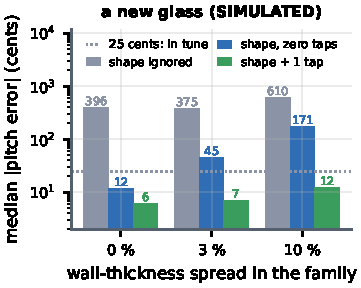
\includegraphics[width=\linewidth]{images/figures/fig_newcontainer.pdf}
    \column{0.49\textwidth}
        \centering
        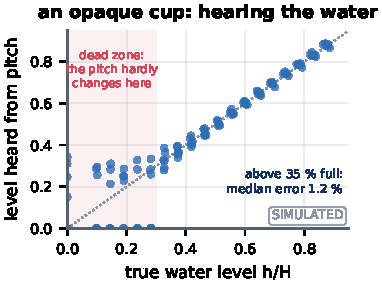
\includegraphics[width=\linewidth]{images/figures/fig_hearlevel.pdf}
    \end{columns}
    \vspace{1mm}
    \scriptsize
    \begin{itemize}
        \item \textbf{A new glass} (left): ignoring its shape, the pitch is \EnineAvg\ cents off; its shape alone gives \EnineZero\ cents
              (\EnineZeroSame\ if all walls are equal); one check tap gives \EnineTap. The hidden wall thickness sets the limit.
        \item \textbf{An opaque cup} (right): one tap when empty, then each tap's pitch gives the level, within \EtenAbove\,\% of the
              height above 35\,\% full. Below 30\,\% the law is too flat: a tap varies more (8 cents) than the water changes it.
        \item The fitted radius exponent is $\EnineExp$, close to French's $-2$: the camera and the taps recover the physics.
    \end{itemize}
\end{frame}
